\nsecbegin{Ziel des Sprints}
Ziel des Sprints ist, ein funktionaler Zustand der Software. Die Bedienung soll möglichst fehlerfrei über GUI und Kommandozeile ermöglicht werden. Des weiteren sollen alte Codefragmente entfernt und die Struktur der einzelnen Klassen weiterhin verbessert werden. Da ein Ende des Projektes langsam absehbar ist, sollen Unit-Tests für eine größere Testüberdeckung sorgen, die einzelnen Teile sowie die Weiterentwicklung der Sequenzdiagramm-Generierung (Exceptions visualisiert) sollen angepasst werden, jedoch keine weitere Grundlegende Funktionalität hinzugefügt werden. \\
Zusätzlich werden weitere Methoden in der XML-Hilfsklasse implementiert und für bessere Fehlerbehandlung der Logger erweitert. Weitere Auswahloptionen für eine verbesserte Nutzerinteraktion sollen in GUI und Konsole implementiert, sowie kleinere Bugfixes vorgenommen werden.\\

% HIER NEUES KLASSENDIAGRAMM HINZUFUEGEN
%\begin{figure}[hbtp]
%\centering
%\includegraphics[scale=0.5]{}
%\caption{Klassendiagramm des Sprints}
%\end{figure}
\nsecend

\nsecbegin{User-Stories des Sprint-Backlogs}
\nsecbegin{Exceptions als Sequenzdiagramme}
Als Benutzer wünsche ich mir, dass der mögliche Pfad der Exceptions als Sequenzdiagramm angezeigt werden kann, um ungehandelte Exceptions zu vermeiden.
\nsecend
\nsecbegin{Klassendiagramme}
Als Benutzer wünsche ich mir, Klassendiagramme aus meinem bestehenden Quellcode erstellen zu können, damit ich das nicht manuell tun muss.
\nsecend
\nsecbegin{Klassenauswahl}
Als Benutzer wünsche ich mir die Möglichkeit, Klassen zu selektieren, damit die Diagramme nicht zu unübersichtlich werden.
\nsecend
\nsecbegin{Kommandozeile}
Als Benutzer wünsche ich mir, dass das Programm von der Kommandozeile aus aufrufbar ist, um es automatisiert starten zu können.
\nsecend
\nsecbegin{Methoden- und Variablenauswahl}
Als Benutzer wünsche ich mir die Möglichkeit, Methoden und Variablen zu selektieren, damit die Diagramme nicht zu unübersichtlich werden.
\nsecend
\nsecbegin{Multiple Klassenauswahl}
Als Benutzer wünsche ich mir einen Button, mit dem ich alle Klassen an- oder abwählen kann, damit ich nicht alle Klassen einzeln auswählen muss.
\nsecend
\nsecbegin{Sequenzdiagramme}
\nsecbegin{Auswahl des zu erstellenden Diagramms}
Als Benutzer wünsche ich mir, dass eine Auswahl zwischen Klassen- und Sequenzdiagrammen möglich ist, damit ich diese je nach meinen Bedürfnissen generieren kann.
\nsecend

\nsecbegin{Generierung von Sequenzdiagrammen}
Als Benutzer wünsche ich mir, Sequenzdiagramme erstellen zu können, um einen Überblick über die Abläufe meines Programms zu erhalten.
\nsecend
\nsecend%Sequenzdiagramme
\nsecend % {User-Stories des Sprint-Backlogs}

\nsecbegin{Zeitliche Planung}
Für die Zeitliche Planung wurde von der ursprünglichen Idee, den Sprint eine Woche dauern zu lassen abgesehen, da ein Feiertag auf das Datum der Zwischenstandspräsentationen fiel. Somit wurde der Sprint 7 vom 07.06.2019 bis zum 17.06.2019 angesetzt.
%\begin{figure}[hbtp]
%\centering
%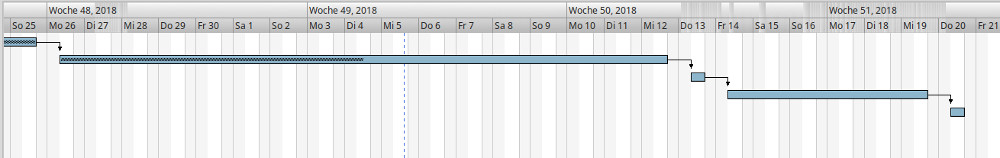
\includegraphics[width=\textwidth]{Bilder/gantt}
%\caption{Gantt-Diagramm für Sprint 1}
%\end{figure}
\nsecend%Zeitliche Planung

\nsecbegin{Liste der durchgeführten Meetings}
\begin{itemize}
\item Planning-Meeting (07.07.2019)
\item Meeting zur Präsentation des Zwischenstands (14.06.2019)
\item Review-Meeting (17.06.2019)
\end{itemize}
\nsecend%Liste der durchgeführten Meetings

\nsecbegin{Ergebnisse des Planning-Meetings}
Neben der Vereinbarung des angestrebten Funktionsumfangs, wurden weitere Bedingungen für Teile der Software zusammengetragen. Damit wurde die Spezifikation wie folgt erweitert:\\
\begin {itemize}
\item Variablen der Basisdatentypen eingefügt
\item Zugriffsmodifikatoren für Instanzen, Variablen und Methoden eingefügt
\item Konstruktor ist nun auch eine Methode in parsedData.xml
\item static-modifier sollte nun geparsed und in Klassendiagramme übernommen werden
\item Alle Methoden die kein Konstruktor sind, haben nun einen Result-Wert (ggf. void)
\item Eigene parsedData.xml für c++
\end {itemize}
Außerdem soll die Software nun auch bei komplexeren Klassendiagrammen ein zuverlässiges Ergebnis liefern. Bezüglich der Sequenzdiagramme soll die Grundfunktionalität erreicht werden, verschachtelte Aufrufe, wie bspw. instanz.methode().methode() oder instanz.methode(instanz.methode) sollen vorerst nicht berücksichtigt werden, jedoch nicht zum Absturz des Programms führen.\\
Die Entwicklung des C++ Parsers wird vorerst auf Klassendiagramme eingeschränkt.\\
Das Anzeigen und Auswählen der Klassen fürs Klassendiagramm in GUI und Konsole sollte funktionieren, sowie das Anzeigen und Auswählen der Eintrittsmethode für das Sequenzdiagramm.
Die Klasse ''ClassDiagrammgenerator'' soll über die boolischen Variablen: showInstances, showVars und showMethods verfügen und von außen gesetzt werden können.
Die Grundlage für die Weiterentwicklung und das Erreichen eines soliden Funktionsumfangs der Software wurde damit gelegt.
\nsecend

\nsecbegin{Aufgewendete Arbeitszeit pro Person$+$Arbeitspaket}
\begin{longtable}{|p{4cm}|l|l|l|l|l|}
        \hline
        Arbeitspaket & Person & Start & Ende & h & Artefakt\\
        \hline
        Console & Marian G. & 07.06.2019 & 17.06.2019 & 23 & Console.java\\ \hline
        Sequenzdiagramm & Tore A.  & 07.06.2019 & 17.06.2019  &20 & SequenceDiagramGenerator.java \\ \hline
        Sequenzdiagramm & Patrick O.  & 07.06.2019 & 17.06.2019  & 4  & SequenceDiagramGenerator.java \\ \hline
        Logger & Patrick O.  & 07.06.2019 & 17.06.2019  & 1  & Logger.java \\ \hline
        Hilfsklasse xml & Leo R.  & 07.06.2019 & 17.06.2019  & 4  & XmlHelperMethods.java \\ \hline
        Klassendiagramm & Johann G.  & 07.06.2019 & 17.06.2019  & 29 & ClassDiagrammGenerator.java \\ \hline
        Hilfsklasse xml  & Patrick O.  & 07.06.2019 & 17.06.2019  & 1 & XmlHelperMethods.java \\ \hline
        C++ Parser  & Jan S.  & 07.06.2019 & 17.06.2019  & 8 & XmlHelperMethods.java \\ \hline
        Java Parser  & Jona M.  & 07.06.2019 & 17.06.2019  & 16 & ParserJava.java \\ \hline
        Java Parser  & Michael L.  & 07.06.2019 & 17.06.2019  & 13 & ParserJava.java \\ \hline
        Unit Tests  & Elisabeth S.  & 07.06.2019 & 17.06.2019  & 14 & *GeneratorTest.java \\ \hline
        Gui  & Julian U. & 07.06.2019 & 17.06.2019  & 8 & GUISwing.java \\ \hline
\end{longtable}     
\nsecend

\nsecbegin{Konkrete Code-Qualität im Sprint}
Durch das Entfernen der Codefragmente, die in nahezu jeder Klasse vorgenommen wurden hat das Projekt an Übersichtlichkeit gewonnen. In einigen Klassen (Konsole bspw.) wurden komplett redundante Codezeilen durch effizientere Lösungen ersetzt und die Wartbarkeit erhöht.
\nsecend%Konkrete Code-Qualität im Sprint

\nsecbegin{Konkrete Test-Überdeckung im Sprint}
Die Testüberdeckung ist mit 62,9\% leicht zurückgegangen, aber noch durchaus im vertretbaren Bereich.
\nsecend%Konkrete Test-Überdeckung im Sprint

\nsecbegin{Ergebnisse des Reviews}
\begin{table}[H]

\begin{tabularx}{\textwidth}{ |l|l|X| }
\hline
\textbf{Klasse} & \textbf{Methode} & \textbf{Anmerkungen}\\
 \hline
XmlHelperMethods & delNode & Löschen eines Knotens aus xml-Dokument, wurde implementiert und getestet\\ \hline
XmlHelperMethods & writeToFile & Generiert XML Datei, wurde implementiert und getestet\\ \hline
XmlHelperMethods & compareXml & Rückgabewert wurde geändert \\ \hline
Sequenzdiagramm & createDiagram & Bugfixes, wurde getestet\\\hline
Logger & LogMain & Auf xml-Struktur umgestellt, korrekt angepasst\\\hline
Gui & showGui & Auflistung der Klassen und Methoden, fehlt\\\hline
ParserJava & parse & Bugs wurden gefixt, weitere Anpassungen ausstehend \\ \hline
Console & interactiveMode & Anpassung auf neue Methoden, Dateiauswahl, Fehlerbehandlung Nutzereingabe, wurde implementiert und getestet. Redundante Zeilen entfernt, Klassenvariablen eingebunden. \\ \hline
ClassDiagramGenerator & createDiagram & Ausgabe von Variablen und Methoden erweitert, wurde implementiert. Boolsche Variablen showInstances, showVars, showMethods fehlen.\\ \hline
\end{tabularx}
\end{table}

Sonstiges:
\begin{itemize}
\item Testabdeckung weiter erhöhen
\item Präsentation (Plakat, Demo) vorbereiten
\item Dritte Zwischenstandspräsentation am 21.06.2019
\end{itemize}
\nsecend%Ergebnisse des Reviews

\nsecbegin{Abschließende Einschätzung des Product-Owners}

\nsecend%Abschließende Einschätzung des Product-Owners

\nsecbegin{Abschließende Einschätzung des Software-Architekten}
Die Sequenzdiagramme können für die Spezifikation über die Kommandozeile erzeugte werden. In der GUI scheint hier noch ein Fehler zu sein. Klassendiagramme für Java funktionieren zuverlässig. Für C++ noch nicht. 
\nsecend%Abschließende Einschätzung des Software-Architekten

\nsecbegin{Abschließende Einschätzung des Team-Managers}
Allgemein kann Sprint 7 als erfolgreicher und produktiver Sprint gewertet werden. Mit 10 geschlossenen Tickets wurde die Entwicklung zu einer stabilen und lauffähigen Version weiter vorangetrieben. Die Bedienbarkeit der Software ist verbessert worden und die Erzeugung von Sequenzdiagrammen ist gegeben. Es bestehen weiterhin kleinere Fehler im Parser und in bei der Erzeugung von Klassendiagrammen. Mit dem nächsten Sprint sollten diese Bugs allerdings behoben werden und die Software wird im vollen Maße einsatzbereit sein.
Positiv anzumerken ist die selbstständige Arbeitsweise aller Teilnehmer, sowie die Zuweisung von Tickets und Nutzung der zur Verfügung stehenden Kommunikationsmittel.
\nsecend%Abschließende Einschätzung des Team-Managers